Funktionsweise der Bildverarbeitung

nachdem der bildausschnitt gewählt wurde, wird das bild wird in Grauwerte umgewandelt. mit der RGB Information kann Fehlerkorrektur gemacht werden.

dann wird jeder blob durch einen Kreis mit der gleichen fläche und dem gleichen schwerpunk ersetzt. auf diesen kreisen kann dann Statistik gemacht weredn. die hoppnug ist dass so unterschiedliche geometieren des schnees abgebieldet werden können. in \ref{} ist der Code der die übersetztung von schwar weiss bildern zu die kreise in eine Datenbank speichern übernimmt.

die auswahl des bildausschnitts und übersetzung in schwarz weiss ist sematisch in \ref{fig:Bildverarbeitnugskonzpet} dargestellt.


\begin{figure}
    \centering
    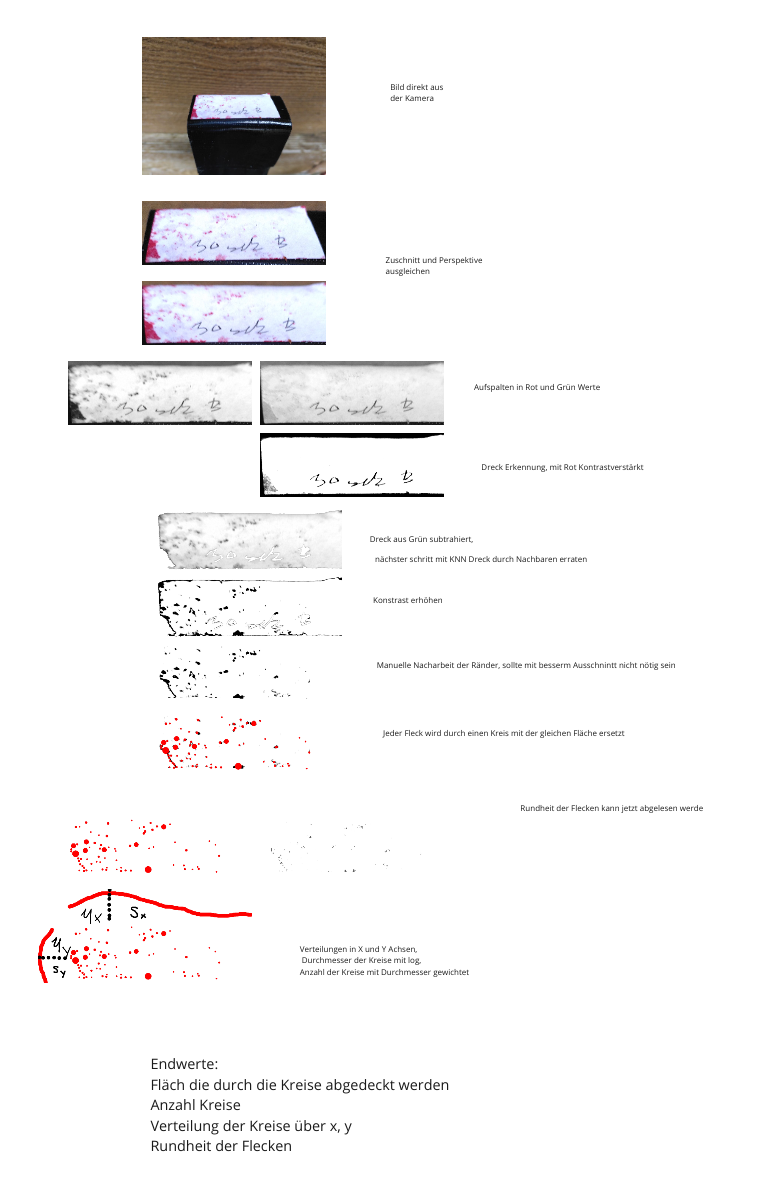
\includegraphics[width=0.8\textwidth]{Bilder/Screenshotfrom2024-04-0112-59-42.png}
    \caption{Bildverarbeitnugskonzpet}
    \label{fig:Bildverarbeitnugskonzpet}
\end{figure}

\newpage
